%label:"art:exactSequencesInSymplecticGeometry"
%author:JeffHicks
%name:"exact sequences in symplectic geometry"
%type:"exposition"

\begin{exposition}
These expository notes are meant to provide some background for how to use exact sequences in Lagrangian intersection Floer cohomology. The notes are largely based on \cite{auroux2014beginner}.
Recall that given Lagrangian submanifolds $L_1, L_2$ which satisfy some suitable hypotheses:
\begin{itemize}
    \item the Lagrangian submanifolds do not bound pseudoholomorphic disks (for example by asking that $\omega(\pi_2(X, L_i))=0$), \label{cond:unobstructed} 
    \item The Lagrangian submanifolds are spin and graded, and\label{cond:orientationgrading}
    \item The intersections between $L_1, L_2$ are transverse. \label{cond:transverseintersection}
\end{itemize}
we can construct a cochain complex called Lagrangian intersection Floer cohomology. As a vector space, this cochain complex is generated on the intersections of our Lagrangian submanifolds
\[\CF(L_0, L_1):= \bigoplus_{x\in L_1\cap L_2} \Lambda\langle x\rangle.\]
Here, $\Lambda$ is the \snip{Novikov ring}{def:novikovRing}.
The differential on this cochain complex comes from the structure constants 
\[\langle d(x), y\rangle:=\sum_{u\in \mathcal M(x, y)}\pm T^{\omega (u)}.\]
In general, this cochain complex is difficult to compute. However, there exist a number of tools whereby geometric relations between Lagrangian submanifolds translate into algebraic relations on their Lagrangian intersection Floer cohomology groups. The natural language for these relations comes from the Fukaya category. Recall that this is a \snip{ $A_\infty$ category}{def:ainfinityCategory} whose: 
\begin{itemize}
    \item objects are Lagrangian submanifolds $L_i$ satisfying the conditions above,
    \item morphism spaces are given by the Lagrangian intersection Floer cochains $\CF(L_0, L_1)$,
    \item Compositions are given by maps 
    \[m^k: \CF(L_{k-1}, L_k)\otimes\cdots \otimes \CF(L_0, L_1)\to \CF(L_0, L_k)[2-k]\]
    which count holomorphic polygons with boundaries on the $L_i$ and corners limiting to their intersection. 
\end{itemize}
%tag:000X
%label:"fig:productConventions"
%author:JeffHicks
%name:"Fukaya product conventions"
%type:"figure"
%parent:"cnv:floerConventions"
%caption:"Conventions for products in the Fukaya category"


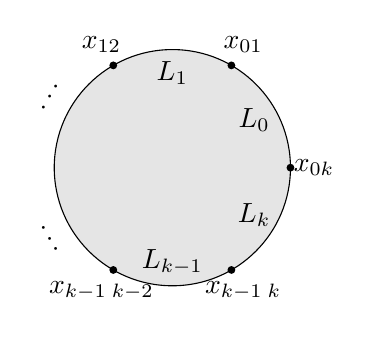
\begin{tikzpicture}

    \draw[fill=gray!20]  (0,0) ellipse (1.5 and 1.5);
    \node at (0:1.8) {$x_{0k}$};
    \node at (30:1.2) {$L_0$};
    \node at (60:1.8) {$x_{01}$};
    \node at (120:1.8) {$x_{12}$};
    \node at (90:1.2) {$L_1$};
    \node[rotate=240] at (150:1.8) {$\dots$};
    
    \node at (-30: 1.2) {$L_k$};
    \node at (-60:1.8) {$x_{k-1\;k}$};
    \node at (-90:1.2) {$L_{k-1}$};
    \node at (-120:1.8) {$x_{k-1 \;k-2}$};
    \node[rotate=-240] at (-150:1.8) {$\dots$};
    
    \node[circle, fill=black, scale=.3] at (0:1.5) {};
    
    \node[circle, fill=black, scale=.3] at (60:1.5) {};
    \node[circle, fill=black, scale=.3] at (120:1.5) {};
    \node[circle, fill=black, scale=.3] at (-60:1.5) {};
    \node[circle, fill=black, scale=.3] at (-120:1.5) {};
    
    \end{tikzpicture}
The goal of this note will be to explain how to leverage additional algebraic structure on the Fukaya category to compute Lagrangian intersection Floer cohomology.

We are motivated by the following strategy.
In other categories, you might try to understand the structure of the category by reducing it to some set of irreducible objects. For instance, if you were studying modules, you might notice that for every map between modules you have a kernel of the map, which is again a module. This process gives you a method for decomposing modules into irreducible modules. 

In the Fukaya category, the morphisms are (linear combinations of) intersection points between Lagrangian submanifolds, so it is unclear how to construct the kernel of a map.
While we do not have access to kernels or cokernels --- and therefore cannot define exact sequences --- we can at least put the structure of a triangulated category on $\Fuk(X)$, which will give us access to tools similar to exact sequences. 

\begin{itemize}
    \item We then look at how to enlarge an $A_\infty$ category to an $A_\infty$ category in \cref{art:triangulatedEnvelopes}. In particular, we will obtain a triangulated enlargement of the Fukaya category, so it will make sense to say things like ``the Lagrangians $L_0, L_1, L_1$ sit in an exact triangle''.
    \item We will then look at several examples (Lagrangian surgery, Dehn Twist, and Lagrangian cobordisms) where exact triangles arise in symplectic geometry.
\end{itemize}
%label:"art:triangulatedEnvelopes"
%author:JeffHicks
%name:"How to make a category triangulated"
%type:"article"

We have no expectation that the geometric Fukaya category $\Fuk(X)$ is triangulated: indeed, it is only guaranteed that the category is \emph{pre-additive}. Never-the-less, we would like to say that $\Fuk(X$) can be enhanced to a triangulated category.
There are general constructions which enlarge an $A_\infty$ category $\mathcal C$ to a triangulated category. These constructions rely on the fact that the $A_\infty$ structure on $\mathcal C$ already knows what its exact triangles should be. 

We give two enlargements: the category of modules over $\mathcal C$, or the category of twisted complexes. These notes are based on Chapter 3 of \cite{seidel2008fukaya}.

%tag:000N
%label:"art:aInfintyModules"
%author:JeffHicks
%name:"The Category of modules over an $A_\infty$ category"
%type:"article"

 Given $\mathcal C$ an $A_\infty$ category, there is a category of $\text{Mod}-\mathcal C$ (dg category of $A_\infty$-modules) which is triangulated.

%tag:000E
%label:def:moduleOveraInfinityCategory
%author:JeffHicks
%name:"Module over an $A_\infty$ category"
%type:definition

 
 
Let $\mathcal A$ be  an \emph{$A_\infty$} category; denote the product structure by $m^k_\mathcal A$. A right $\mathcal A$ module (denoted by $M\in \text{Mod}-\mathcal A$ is a 
\begin{itemize}
    \item assignment $M(A)$ of a graded module to each $A\in \text{Ob}(\mathcal A$) and,
    \item for sequence $A_0, \ldots, A_k$ of objects in $\mathcal A$, a composition map 
    \[
        m^{1|k}_{M|\mathcal A}:M(A_k)\otimes \hom(A_{k-1}, A_k)\otimes \cdots \otimes \hom(A_1, A_0)\to M(A_k)[1-k]
    \]
for each $k\geq 0$. 
\end{itemize}
These are required to satisfy the quadratic  $A_\infty$ relationships:\todo{check this}
\begin{align*}
    0=&\sum_{\substack{ j_1+j+j_2=k_1+1\\j_1>0 }} m_{M|{\mathcal A}}^{1|k_1-j+1}\circ ( \operatorname{id}_M\otimes  \operatorname{id}_A^{\otimes j_1}\otimes m^{j}_A \otimes \operatorname{id}^{\otimes k_1-j_1-j})\\
    &+\sum_{\substack{ j+j_2=k_1+1\\j_1\leq k_1\leq j_1+j-1}} m_{M|\mathcal A}^{1|j_2} \circ (m_{A|M}^{1|j}\otimes  \operatorname{id}_A^{\otimes j_2})
\end{align*}

 
%label:"exm:ringModule"
%name:"modules over a ring as $A_\infty$ modules"
%type:"example"

The name module comes from the simplest example. Let $R$ be a ring. Now consider the $A_\infty$ category $\mathcal A$ which only contains one object $A$, and $\hom(A, A)=R$. 

Let $M$ be an $R$-module. We obtain a $\text{mod}-\mathcal A$ with the assignment $M(A)=M$,  and whose product $m^{1|k}:M(A)\tensor A^{\tensor k}\to M(A)$ is 
\[
    m^{1|1}(x,r)=x\cdot r
\]
and vanishes if $k\neq 1$. The $A_\infty$ module relations state 
\[m^{1|1}(m^{1|1}(x, r_1),r_2)-m^{1|1}(x, m^2(r_1, r_2))=(x\cdot r_1)\cdot r_2 - x\cdot (r_1\cdot r_2)=0\]
which is guaranteed by associativity of the product. 

Given any chain complex of $R$-modules $M^\bullet$, we similarly obtain a right $\mathcal A$ module by taking $M^\bullet(A)=M^A$; the $A_\infty$ module relations now state that $m^{1|0}\circ m^{1|0}= d_M\circ d_M=0$, and that $d_M$ is a morphism of $R$-modules.

There are right $\mathcal A$-modules beyond chain complexes. However, given any right $\mathcal A$-module, the homology of the complex $H^\bullet(M(A))$ is a graded $R$-module.
%label:"exm:zeroModule"
%name:"$A_\infty$ zero module"
%type:"example"

Let $\mathcal A$ be an $A_\infty$ category. We can define the zero module $M$ which has the property that for all $A\in \mathcal A$, our module assigns $M(A)=0$. As a result, the composition maps $m^{1|k}$ all vanish. This trivially satisfies the quadratic $A_\infty$ module relations.

While this appears to be a artificial example, it is generally desirable to have a zero object in your category, and there is no reason a priori for your original $A_\infty$ category $\mathcal A$ to have a zero object. For the example we are interested--- the Fukaya category--- there is no ``zero'' Lagrangian submanifold.
%label:"exm:yonedaModule"
%name:"$A_\infty$ Yoneda module"
%type:"example"

Let $\mathcal A$ be an $A_\infty$ category. Let $A\in \mathcal A$ be an object. We can associate to $A$ the \emph{Yoneda module}, $\mathcal Y_A$, which on every object $B\in \mathcal A$ assigns the chain complex
\[\mathcal Y_A(B):=\hom(B, A),\]
and whose product maps are defined by 
\[m^{1|k-1}(m,a_{k-1}, \ldots, a_0):= m^k(m,a_{k-1}, \ldots, a_0).\]
Note that the $A_\infty$ module relations for $Y_A(B)$ are exactly the $A_\infty$ product relations for $\mathcal A$.
\label{exm:yonedaModule}

%tag:000L
%label:"def:morphismOfaInfinityModules"
%author:JeffHicks
%name:"morphism of $A_\infty$ modules"
%type:"definition"
%status:"incomplete"
  
Let $M, N$ be $A_\infty$ modules. A  \emph{pre-morphism of $A_\infty$ modules} of degree $d$ is a collection of maps $f^{1|k-1}: A^{\otimes k-1}\otimes M\to N[d-k+1]$. The set of pre-morphisms, $\hom^\bullet(M, N)$ is a cochain complex whose differential is
\[(m^1_{\hom^\bullet(M, N)} f)^{k-1, 1}\]

 
%tag:000E
%label:"def:categoryOfAInfinityModules"
%author:JeffHicks
%name:"category of $A_\infty$ modules"
%type:"definition"

 
 
Let $\mathcal A$ be  an \emph{$A_\infty$} category. The \emph{category of right $\mathcal A$- modules}, denoted by $\text{Mod}-\mathcal A$, is the differential graded category whose: 
\begin{itemize}
    \item Objects are right $\mathcal A$ modules and
    \item chain complexes of morphisms are the chain complexes of $\mathcal A$ module pre-morphism,
    \item composition is given by 
    \[m^2_{\text{mod}-\mathcal A}(f, g)=\sum_{j+j_2=k}-(-1)^\diamondsuit f^{1|j_2}(g^{1|j-1}\tensor \id^{j^2})\]
    \item higher product vanishing for $k\geq 3.$
\end{itemize}
 
%label:"prp:aInfinityModulesIsDG"
%author:JeffHicks
%name:"dg-category structure on $\mathcal A-\text{Mod}$"
%type:"proposition"

 
 Let $\mathcal A$ be an $A_\infty$ category. The category of modules over $\mathcal A$ has the structure of a dg-category.

 
One observes that $\mod-\mathcal A$ is in general a ``nicer'' category than $\mathcal A$, as it inherits many of the properties of the category of chain complexes.
%label:"prp:categoryOfAInfinityModulesIsTriangulated"
%author:JeffHicks
%name:"triangulated structure on $\mathcal A-\text{Mod}$"
%type:"proposition"

 
 
Let $\mathcal A$ be  an \emph{$A_\infty$} category. Then $H^0(\text{mod}-\mathcal A)$ is a triangulated category.

 
%label:"prf:categoryOfAInfinityModulesIsTriangulated"
%author:JeffHicks
%name:"proof that the category of $A_\infty$ modules is triangulated"
%type:"proof"
%parent:"prp:categoryOfAInfinityModulesIsTriangulated"

 
 
We only describe the exact triangles in the category. Given $f\in \hom(M, N)$ a morphism of right $A_\infty$ modules, we define the cone module to be 
\[\cone(f)(A):=M(A)\oplus N(A)[1]\]
whose $A_\infty$ module structure is given by 
\[ m^{1|k}_{\cone(f)|\mathcal A}:=m^{1|k}_{M|\mathcal A}\oplus (f^{1|k}+ m^{1|k}_{N|\mathcal A}).\]

 
The Yoneda module construction (\cref{exm:yonedaModule}) gives a fully faithful contravariant functor $\mathcal A \to \mod-\mathcal A$.
As the category $\mod-\mathcal A$ has mapping cones, this gives a triangulated envelope for $\mathcal A$.
We therefore say that $A\to B \to C$ is an exact triangle in $\mathcal C$ if the image under Yoneda embedding is isomorphic to $A\to B \to \cone(f)$.


%label:"art:twistedComplexes"
%author:JeffHicks
%name:"the category of twisted complexes"
%type:"article"


One viewpoint on mapping cones of cochain  complexes is that they give \emph{deformations} of (direct sums of) objects of our categories. Given a map of cochain complexes $f: A\to B$, the differential on $\cone(f)$ has the form 
\[d_{\cone(f)}=\begin{pmatrix} d_A & 0 \\ 0 & d_B \end{pmatrix} + \begin{pmatrix} 0 & 0\\ f & 0\end{pmatrix}\]
where the first term is the differential on $A\oplus B[1]$, and the second term ``deforms'' the differential on this chain complex.

Twisted complexes  extend this story in several directions: firstly, we expand the set of deformations so that the objects we consider are chain complexes up to homotopy, and we allow deformations of the product (and not only differential) structure.

%label:"def:twistedComplex"
%author:JeffHicks
%name:"twisted complex"
%type:"definition"

 
 
Let $\mathcal C$ be an $A_\infty$ category. A twisted complex $(E, \delta_E)$ consists of:
\begin{itemize}
\item $E$, a formal direct sum of shifts of objects
\[E:=\bigoplus_{i=1}^N E_i[k_i]\]
where $E_{i}\in Ob(\mathcal C)$, and $k_i\in \ZZ$.
\item  A differential $\delta_E$, which can be written as a matrix  of degree 1 maps
\[\delta^{ij}_E: E_i[k_i]\to E_j[k_j +1] .\] These maps must satisfy the following conditions:
\begin{itemize}
    \item the matrix $\delta_E$ is strictly upper triangular and;
    \item They satisfy the Maurer-Cartan relation:
    \[\sum_{k\geq 1} m^k (\delta_E\otimes\cdots \otimes \delta_E) =0.\]
\end{itemize}
\end{itemize}

 

%tag:000R
%label:"rem:twistedComplexConvergence"
%author:JeffHicks
%name:"convergence in twisted complexes"
%type:"remark"


The condition that the matrix $\delta_E$ is strictly upper triangular is to ensure that the sum in the Maurer-Cartan relation converges. One can also ask that there exists a filtration on $E$, the formal direct sum of shifts of objects, and that the differential $\delta_E$ respects the filtration (see Section 31 of \cite{seidel2008fukaya}). From this perspective, the twisted complex looks more like a formal deformation of the direct sum.
 
%tag:000R
%label:rem:twistedComplex
%author:JeffHicks
%name:"properties of twisted complexes"
%type:remark

 


    One viewpoint on twisted complexes is that they give \emph{deformations} of (direct sums of) objects of our categories. In the simplest case --- the mapping cone of chain map $f: A\to B$, the differential on $\cone(f)$ has the form 
    \[d_{\cone(f)}=\begin{pmatrix} d_A & 0 \\ 0 & d_B \end{pmatrix} + \begin{pmatrix} 0 & 0\\ f & 0\end{pmatrix}\]
    where the first term is the differential on $A\oplus B[1]$, and the second term ```deforms'' the differential on this chain complex.

    Twisted categories extend this story in several directions: firstly, we expand the set of deformations so that the objects we consider are chain complexes up to homotopy, and we allow deformations of the product (and not only differential) structure.

    With regards to the first point: Suppose that we have a (not necessarily exact) sequence of chain complexes $A\xrightarrow{f} B \xrightarrow{g} C$. The total complex of this sequence will not be a chain complex (as $g\circ f \neq 0$). However, to build a twisted complex from this data we will only need that $g\circ f$ is homotopic to zero. Suppose that  $H:A\to C[1]$ is a homotopy (so that $d_AH+Hd_C=g\circ f$). Then  
    \[\delta = \begin{pmatrix}
        0 & 0 & 0\\
        f & 0 & 0\\
        H & g & 0
    \end{pmatrix}\]
    gives us the structure of a twisted complex on $A\oplus B[1]\oplus C[2]$.

    For the second point: Let $(A, m^k)$ be an $A_\infty$ algebra. There are a particularly nice class of deformations of $A_\infty$ governed by elements $a\in A^1$ satisfying the Maurer-Cartan equation:
    \[m^1(a)+m^2(a\otimes a)+m^3(a\otimes a \otimes a)+\cdots =0.\]
    In order for this equation to make sense, one needs show that the sum converges. This is usually achieved by asking that $A$ be filtered and that $m^k(a^{\otimes k})$ lies increasingly positive filtration levels.
    When one can make sense of this equation, we can define a new $A_\infty$ algebra, $(A, m^k_a)$ whose product is defined by 
    \[m^k_a:=\sum_{n>0}\sum_{j_0+\cdots+j_k=n} m^{k+n}(a^{\otimes j_0}\otimes \id \otimes a^{\otimes j_1}\otimes \id \cdots \otimes a^{\otimes j_{k-1}}\otimes \id \otimes a^{\otimes j_k})\]

    Now consider the setting where $C$ is a chain complex, and $A=\hom(C, C)$. Then $a\in A^1$ corresponds to a map $a: C\to C[1]$, and the Maurer-Cartan equation has two terms:
    \begin{itemize}
        \item The first term $m^1(a) = d_A a + a d_A$. The vanishing of this term states that $a$ is a chain map;
        \item The vanishing of the second term $m^2(a, a)$ tells us that $a$ squares to zero (so that it gives a differential).
    \end{itemize}
    The combination of these two terms checks the condition that $(d_A+a)\circ (d_A+a)=0$; that is that we can deform the differential by $a$.
 
%tag:000S
%label:"def:morphismOfTwistedComplexes"
%author:JeffHicks
%name:"morphism of twisted complexes"
%type:"definition"

 
 
Let $(E, \delta_E)$ and $(F, \delta_F)$ be two twisted complexes. A \emph{morphism of twisted complexes} is a collection of morphisms 
\[f_{ij}:E_i[k_i]\to E_j[k_j],\]
so that $\hom^d((E, \delta_E), (F, \delta_F))=\bigoplus_{i, j}\hom^{d+k^F_j-k^E_i}(E_i, F_j).$
Given a sequence $\{(E_i, \delta_i)\}_{i=0}^k$ of twisted complexes, and $a_i\in\hom^d((E_{i-1}, \delta_{E_{i-1}}), (E_{i}, \delta_{E_{i}}))$, we have a composition 
\[m^k_{\operatorname{Tw}}(a_{k}\otimes \cdots \otimes a_{1} ):=\sum_{j_0, \ldots, j_k\geq 0} m^k(\delta_k^{\otimes j_k}\otimes a_{k}\otimes \delta_{k-1}^{\otimes j_{k-1}}\otimes a_{k-1}\otimes \cdots \otimes a_1\otimes \delta_0^{\otimes j_{0}}().\]

 
%label:"prp:categoryOfTwistedComplexes"
%author:JeffHicks
%name:"category of twisted complexes"
%type:"proposition"

 
 
Let $\mathcal C$ be an $A_\infty$ category. The category of twisted complexes, $\operatorname{Tw}(\mathcal C)$, is the $A_\infty$ category whose objects are twisted complexes, morphisms are morphisms of twisted complexes, and $A_\infty$ compositions are given by $m^k_{\operatorname{Tw}}$.

 
%tag:000U
%label:thm:categoryOfTwistedComplexesIsTriangulated
%author:JeffHicks
%name:"twisted complexes form a triangulated category. "
%type:theorem


Let $\mathcal C$ be an $A_\infty$ category. The category of twisted complexes, $\operatorname{Tw}(\mathcal C)$ is a triangulated category. There is a fully faithful inclusion $\mathcal A\to \operatorname{Tw}(\mathcal C)$. Furthermore, the image of $\mathcal A$ generated $\operatorname{Tw}(\mathcal C)$.

%tag:000U
%label:"prf:categoryOfTwistedComplexesIsTriangulated"
%author:JeffHicks
%name:"twisted complexes form a triangulated category. "
%type:"proof"
%parent:thm:categoryOfTwistedComplexesIsTriangulated
%completeness:5

 
 To give twisted complexes the structure of a triangulated category, we must specify what the exact triangles are. Given a morphism $f: (E, \delta_E)\to (F, \delta_F)$, we can define the cone of $f$ to be the twisted complex $(E[1]\oplus F, \delta')$ where $\delta'$ is the matrix
 \[
    \left(\begin{array}{c|c} \delta_E &0 \\ \hline f^ \delta_F \end{array}\right).
\]

 
There exists an inclusion functor $i:\mathcal C\to \Tw(\mathcal C)$.
We can therefore declare that the triangle $A\to B\to C$ is exact in  $\mathcal A$ is if $C$ is quasi-isomorphic to $\cone(A\to B)$ in the category of twisted complexes. 



%label:"art:modulesVsTwistedComplexes"
%author:JeffHicks
%name:"modules or twisted complexes?"
%type:"article"

Both \cref{def:moduleOveraInfinityCategory} and \cref{def:twistedComplex} provide a method for identifying the exact triangles of $\mathcal C$, an $A_\infty$ category. We now highlight some of the differences between these two constructions.

These differences are most easily seen by reducing to a simple setting. Consider $R$ a field. Then the category of twisted complexes over $R$ will be the category of finite dimensional graded vector spaces with a choice of basis, while $\text{mod} R$ will be the category of $R$-vector spaces. Given another ring $S$, and a ring homomorphism $R\to S$, we obtain a map from $\Tw(R)\to \Tw(S)$ and a map $\text{mod}-S\to \text{mod} R$. Also observe that the category of $R$-vector space is much larger than the category of finite-dimensional graded vector spaces.

The construction of twisted complexes is a functor on the category of $A_\infty$ categories,
\[\Tw:A_\infty-\text{cat}\to A_\infty-\text{cat}.\]
The $\text{mod}-\mathcal C$ construction gives us a contravariant functor on the category of $A_\infty$ categories,
\[\text{mod}-(-):A_\infty-\text{cat}\to (A_\infty-\text{cat})^{\text{op}}.\]

For the purposes of computations in symplectic geometry, it is usually unimportant if we consider enlarging the Fukaya category by looking at modules or at twisted complexes, as both structure give us access to the exact triangles in $\Fuk(X)$. Many proofs become cleaner to write when using the viewpoint of $\text{mod}-\mathcal A$, while it can be notationally easier to perform computations using twisted complexes. 

However, if we wish to compare the Fukaya category of a symplectic manifold to some other category (as in the setting of homological mirror symmetry) the choice of triangulated envelope becomes important. In mirror symmetry, we compare the Fukaya category of a symplectic manifold $X^A$ to the derived category of coherent sheaves on a mirror space $X^B$. When $X^B$ is a compact smooth complex variety, this is the same as the category of perfect complexes -- which are precisely the sheaves which can build out line bundles via the operations of taking mapping cones. For this reason, it is more common to see that Fukaya category defined to be the twisted complexes on the geometric Fukaya category in papers related to mirror symmetry.



%label:"art:lagrangianSurgery"
%author:JeffHicks
%name:"surgery of Lagrangian submanifolds "
%type:"article"

%label:"con:polterovichSurgery"
%author:JeffHicks
%name:"Lagrangian connect sum "
%type:"construction"

We will now look at some ways to glue together new Lagrangian submanifolds from old.
A source of inspiration for us will be from smooth topology, where tools such as surgery, Morse theory, and cobordisms provide methods for generating new manifolds.
An example where we can take a method from topology and directly import it into symplectic geometry is connect sum for Lagrangian curves inside of surfaces.
In this setting, two Lagrangian curves which intersect at a point are modified at the point of intersection to produce a connected Lagrangian submanifold.
See \cref{fig:polterovichSurgery}.

The Polterovich connect sum is a generalization of this surgery to higher dimensions, which smooths out a transverse intersection between two Lagrangian submanifolds. 
The idea of construction is to take a  \snip{standard model for the transverse intersection}{lemma:straightening}, then construct a model neck in that canonical neighborhood. 
%tag:000X
%label:"fig:polterovichSurgery"
%author:JeffHicks
%name:"Polterovich Surgery"
%type:"figure"
%parent:prp:polterovichSurgery
%caption:"The connect sum of two Lagrangian curves in a surface"

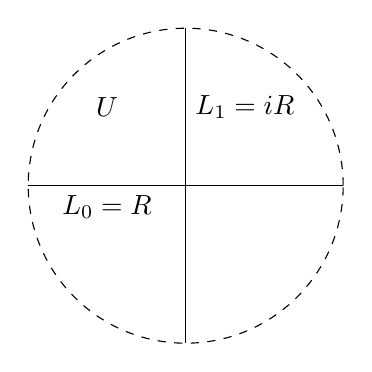
\begin{tikzpicture}
      \draw[dashed]  (0,0) circle[radius=2];
      \draw (-2,0) -- (2,0) (0,2) -- (0,-2);
      \node at (-1,1) {$U$};
      \node[right] at (0,1) {$L_1=i\mathbb R$};
      \node[below] at (-1,0) {$L_0=\mathbb R$};
      \end{tikzpicture}
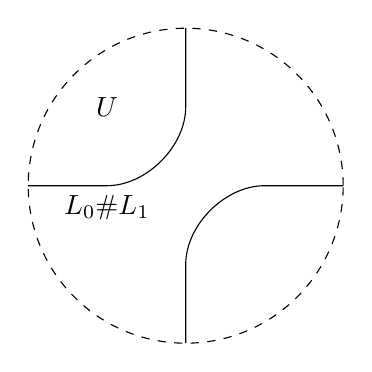
\begin{tikzpicture}
      \draw[dashed]  (0,0) circle[radius=2];
      \node at (-1,1) {$U$};
      
      \node[below] at (-1,0) {$L_0\#L_1$};
      
      \draw (-2,0) .. controls (-1.5,0) and (-1.5,0) .. (-1,0) .. controls (-0.5,0) and (0,0.5) .. (0,1) .. controls (0,1.5) and (0,1.5) .. (0,2) ;
      \draw (2,0) .. controls (1.5,0) and (1.5,0) .. (1,0) .. controls (0.5,0) and (0,-0.5) .. (0,-1) .. controls (0,-1.5) and (0,-1.5) .. (0,-2);
      
\end{tikzpicture}

%tag:000T
%label:"prp:polterovichSurgery"
%author:JeffHicks
%name:"Polterovich surgery of Lagrangian submanifolds"
%type:"proposition"
%source:"polterovich1991surgery"

Let $L_1, L_2\subset X$ be two Lagrangian submanifolds intersecting transversely at a single point $p$. 
Then there exists a Lagrangian submanifold $L_1\#_p L_2\subset X$ which
\begin{itemize}
        \item topologically is the connect sum of $L_1$ and $L_2$ at $p$. 
        \item Agrees with $L_1\cup L_2$ outside of a small neighborhood of $p$ in the sense that 
        \[L_1\#_p L_2|_{X\setminus U}=L_2\cup L_2|_{X\setminus U}.\]
\end{itemize}
 
%tag:000L
%label:"prf:polterovichSurgery"
%author:JeffHicks
%name:"construction of Polterovich surgery"
%type:"proof"
%parent:prp:polterovichSurgery

 
 

By \cref{lemma:straightening}, it suffices to construct the Lagrangian surgery neck replacing the a standard intersection neighborhood $X=\CC^n$, $L_1=\RR^n$ and $L_2=\jmath\RR^n$.
We start by picking a \emph{surgery profile curve},  
\begin{align*}
      \gamma: [-R, R] \to& \CC\\
      t\mapsto& (a(t)+\jmath b(t))
\end{align*}
with the property that $a(t), b(t)$ are non-decreasing, $\gamma(t)=t$ for $t$ sufficiently small, and $\gamma_\lambda(t)=\jmath t$ for $t$ sufficiently large. We ask that the area between the real axis, imaginary axis, and $\gamma$ is $\lambda$.
An example is drawn in \cref{fig:polterovichSurgeryProfile}.
\input{fig_polterovichSurgeryProfile}
This neck provides a local model for the Lagrangian surgery, which is the Lagrangian surgery neck:
\[
	L_1\#_\gamma L_2:=\left\{(\gamma(t)\cdot x_1,\ldots,  \gamma(t)\cdot x_n \text{ such that } x_i \in \RR^n,t\in \RR, \sum_{i} x_i^2=1\right\}.
\]
Note that when $t$ is sufficiently small this parameterizes $(\RR\setminus B_r(0))\subset \CC^n$, and when $t$ is sufficiently large this parameterizes $(\jmath \RR \setminus B_r(0))\subset \CC^n$. 
Therefore, this construction satisfies the condition that the surgery Lagrangian agrees with the surgery components outside of a small neighborhood of the surgery point.
This Lagrangian has the topology of $S^{n-1}\times \RR$, which is the local model for the connect sum $\RR^n\#_0\RR^n$.

It remains to show that the submanifold is Lagrangian \todo{}


The Lagrangian is then taken to be $L_1\#_\gamma L_2$ for any suitable choice of $\gamma$.
 
The order of the summands plays an important role in Lagrangian surgery, as rarely are the Lagrangian $L_1\#L_2$ and $L_2\#L_1$ isotopic. 

The surgery construction does not uniquely specify \emph{the} Lagrangian surgery of two Lagrangian submanifolds,  different choices of curves $\gamma$ produce different Lagrangian submanifolds.
Given a Lagrangian isotopy $\li_t: L\to C$ we associate \snip{flux cohomology class}{def:flux} $\Flux_{\li_t}\in H^1(L)$. 
We can similarly associate a flux class to a Lagrangian surgery.
A given surgery profile curve $\gamma$ can be extended to a family of Lagrangian surgery profiles by scaling the profile curve by a parameter $s$.  
This gives us a family of surgeries $L_1\#_{s\gamma} L_2$, which are Lagrangian isotopic.
The flux of the surgery is defined to be the flux of this isotopy. 
%label:"prp:fluxOfSurgery"
%author:JeffHicks
%name:"flux of Polterovich surgery"
%type:"proposition"

Let $L_0, L_1$ be two Lagrangian submanifolds which intersect transversely at a point, and let $U$ be a neighborhood of the point in which we implant a surgery neck. Suppose two profile curves $\gamma_0, \gamma_1$ have the same flux $\lambda$.
Then there exists a Hamiltonian supported on $U$ whose time one identifies $L_1\#_{\gamma_0} L_2$ and $L_1\#_{\gamma_1} L_2$.
The flux of $\gamma$ is the area bounded by $\gamma$ and the two axis. This is sometimes called the width or neck-width of the surgery.
We will write $L_1\#_{\lambda}L_2$ a Lagrangian connect sum determined by a surgery profile curve with flux $\lambda$.

%label:"exm:polterovichSurgery"
%author:JeffHicks
%name:"Polterovich surgery in $\RR^n$"
%type:"example"


We now visualize the Polterovich surgery for Lagrangian sections of $T^*\RR^n$.
The Lagrangians which we consider are two sections of the cotangent bundle. 
Let $L_1$ be the graph of $d(q_1^2+ \cdots+ q_n^2)$, and let $L_2$ be the graph of $d(-q_1^2-\cdots -q_n^2)$. 
In dimension 2, we can then draw $L_1\# L_2$ and $L_2\# L_1$ as multisections of the cotangent bundle. 
These multisections are sketched in \cref{fig:surgeryDim4}.
Note that one of surgeries creates a Lagrangian which has a ``neck'' visible in the projection to the base of the cotangent bundle.
The other surgery is generically a double-section of the cotangent bundle, except over the fiber of the intersection point where it is instead an $S^1$.


\input{fig_surgeryDim4}


 


%tag:000U
%label:"art:surgeryExactTriangle"
%author:JeffHicks
%name:"the Lagrangian surgery exact triangle "
%type:"article"



Now that we have a geometric description of $L_1\#_\lambda L_2$, we discuss what object it represents in the Fukaya category. We restrict ourselves to $\dim_\RR(X)=2$ so that we may draw pictures. However, the pictures are only for intuition (and in fact the sketch of proof we give only work when $\dim(X)\geq 4$).

Let $L_0$ be some test Lagrangian, which intersects both $L_1$ and $L_2$ as in \cref{fig:roundingCorner}. If the surgery neck is chosen to lie in a neighborhood disjoint from the intersections  $L_0\cap (L_1\cup L_2)$, then these intersections are in bijection with the intersections $L_0\cap (L_1\# L_2)$. Therefore $\CF(L_0, L_1\# L_2)=\CF(L_0, L_1)[1]\oplus \CF(L_, L_2)$ as vector spaces.
%label:"fig:roundingCorner"
%author:JeffHicks
%name:"rounding corner in Polterovich surgery"
%type:"figure"
%parent:"thm_roundingCorner"
%caption:"By rounding the corner, we can compare holomorphic triangles with holomorphic strips on the surgery."


    
    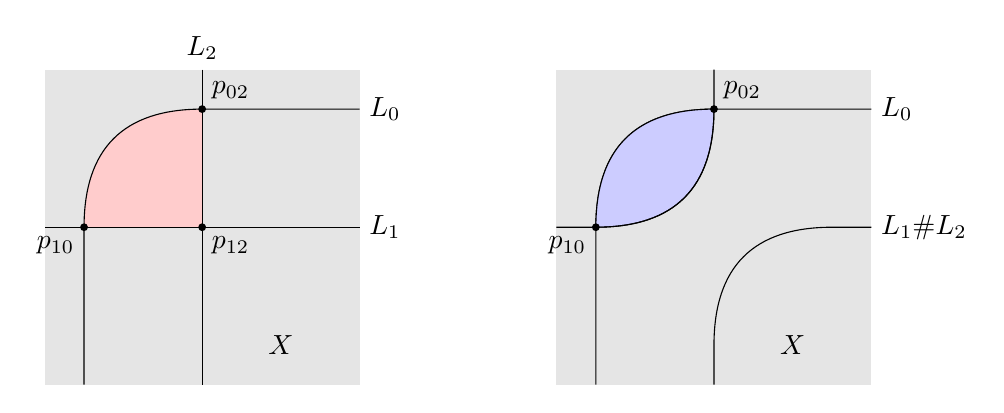
\begin{tikzpicture}\begin{scope}[]
    
    
        \fill[gray!20]  (-2,2) rectangle (2,-2);
        \fill[red!20] (0,0) .. controls (0,0.5) and (0,1) .. (0,1.5) .. controls (-1,1.5) and (-1.5,1) .. (-1.5,0) .. controls (1,0) and (0.5,0) .. (0,0);
        
        \draw (0, 2)--(0,-2);
        \draw (2,0) -- (-2,0);
        \draw (2,1.5) .. controls (1,1.5) and (0.5,1.5) .. (0,1.5) .. controls (-1,1.5) and (-1.5,1) .. (-1.5,0) .. controls (-1.5,-0.5) and (-1.5,-1.5) .. (-1.5,-2);
        
        \node[right] at (2,1.5) {$L_0$};
        \node[right] at (2,0) {$L_1$};
        \node[above] at (0,2) {$L_2$};
        \node[below right] at (0,0) {$p_{12}$};
    \node[above right] at (0,1.5) {$p_{02}$};
    \node[below left] at (-1.5,0) {$p_{10}$};
        \node[fill=black, circle, scale=.3] at (0,0) {};
        \node[fill=black, circle, scale=.3] at (0,1.5) {};
        \node[fill=black, circle, scale=.3] at (-1.5,0) {};
    \node at (1,-1.5) {$X$};
    \end{scope}
        
        
        \begin{scope}[shift={(6.5,0)}]
        
        
        \fill[gray!20]  (-2,2) rectangle (2,-2);
        \draw (2,1.5) .. controls (1,1.5) and (0.5,1.5) .. (0,1.5) .. controls (-1,1.5) and (-1.5,1) .. (-1.5,0) .. controls (-1.5,-0.5) and (-1.5,-1.5) .. (-1.5,-2);
        
        \node[right] at (2,1.5) {$L_0$};
        \node[right] at (2,0) {$L_1\#L_2$};
        
        
        \draw[fill=blue!20] (0,1.5) .. controls (0,0.5) and (-0.5,0) .. (-1.5,0) .. controls (-1.5,1) and (-1,1.5) .. (0,1.5);
        
        \draw (0,2) .. controls (0,1.5) and (0,2) .. (0,1.5) .. controls (0,0.5) and (-0.5,0) .. (-1.5,0) .. controls (-2,0) and (-2,0) .. (-2,0);
        \draw (0,-2) .. controls (0,-2) and (0,-2) .. (0,-1.5) .. controls (0,-0.5) and (0.5,0) .. (1.5,0) .. controls (2,0) and (2,0) .. (2,0);
        
        
    \node[above right] at (0,1.5) {$p_{02}$};
    \node[below left] at (-1.5,0) {$p_{10}$};
        \node[fill=black, circle, scale=.3] at (0,1.5) {};
        \node[fill=black, circle, scale=.3] at (-1.5,0) {};
    \node at (1,-1.5) {$X$};
        \end{scope}
        
        \end{tikzpicture}
 The intuition from \cite{fukaya2007lagrangian} is that there is a bijection between certain holomorphic triangles with boundary on $L_0, L_1, L_2$ which passes through the intersection point $p_{12}$, and holomorphic strips with boundary on $L_0$ and $L_1\# L_2$. Since holomorphic triangles contribute to the $\emprod^3$ structure coefficients, and strips to the differential, it is reasonable to hope that we can state a relation between $L_1, L_2,$ and $L_1\#L_2$ as objects of the Fukaya category.


First, we observe that the intersection point $p_{12}$ determines a morphism in $\hom(L_2, L_1)$. Since we've assumed that $L_1$ and $L_2$ intersect at only one point, we know that $\emprod^1(p_{12})=0$. We can therefore form the twisted complex $\cone(p_{12})$. We now provide justification for why this is isomorphic to $L_1\# L_2$.

We have already observed that for our test Lagrangian $L_0$ we had an isomorphism of vector spaces between $\hom(L_0, L_1)\oplus \hom(L_0, L_2)$ and $\hom(L_0, L_1\#_\lambda L_2)$. The differential on $\hom(L_0, L_1\#_\lambda L_2)$ comes from counting holomorphic strips, which we break into two types: those which avoid a neighborhood of the surgery neck, and those which pass through the surgery neck. 
%label:prp:stripsInLagrangianSurgery
%name:"strips with boundary on Lagrangian surgery avoiding the neck"
%type:proposition


If $\dim_\RR(X)\geq 4$, then we can choose an almost complex structure $J$ so that whenever $p_{01}, q_{01}\in L_0\cap L_1$ are intersections, and $u: [0,1]\times \RR\to X$ is a $J$ holomorphic strip, then the boundary of $u$ is disjoint from a small neighborhood of $L_1\cap L_2$. In particular, $u$ gives a $J$-holomorphic strip with boundary on $L_0, L_1\#_{p_{12}} L_2$.

The more difficult portion is to understand the strips which pass through the neck.
%label:"thm:roundingCorner"
%author:JeffHicks
%name:"rounding the corner"
%type:"theorem"
%source:"fukaya2007lagrangian"


    Let $\dim(X)\geq 4$, and $L_1, L_2$ be exact Lagrangian submanifolds which intersect transversely at a single point $p_{12}$. Let $L_0$ be another exact Lagrangian submanifold which intersects $L_1, L_2$ transversely. Then for sufficiently small surgery necks, there exists a choices of almost complex structure on $X$ for which we have a bijection between
    \begin{itemize}
        \item $J$-holomorphic strips with boundary on $L_0, L_1\# L_2$ which pass through the surgery neck;
        \item $J$-holomorphic triangles with boundary on $L_0, L_1, L_2$.
    \end{itemize}

In fact, \cite{fukaya2007lagrangian} proves the above statement in much greater generality than we state here. The condition that $\dim(X)\geq 4$ can already be seen in in \cref{fig:roundingCorner}. Observe that if we have a pseudoholomorphic triangle whose boundary passes through the point $p_{12}$ in the wrong way, that there is no corresponding pseudoholomorphic strip with boundary on $L_0$ and $L_1\# L_2$.
Ignoring the potential complications in the definition of the Fukaya category, we obtain:
%label:cor:surgeryExactTriangle
%author:JeffHicks
%name:"surgery exact Triangle"
%type:corollary
%

\begin{corollary}
    Let $\dim(X)\geq 4$, and $L_1, L_2$ be Lagrangians which intersect transversely at a single point $p_{12}$. Then $L_1\#_{\lambda} L_2$ is isomorphic to the twisted complex $(L_1[1]\oplus L_2, \emprod^2(p_{12}-)).$
\end{corollary}

%tag:000Y
%label:"art:dehnTwists"
%author:JeffHicks
%name:"symplectic Dehn twist"
%type:"article"

Let $Y$ be a symplectic manifold, and let $S^{n}\subset Y$ be a Lagrangian sphere. 
We now describe a symplectomorphism called \emph{symplectic Dehn twist:}
\[\tau_{S^n}: Y\to Y,\]
described in \cite{seidel2003long}. 
%tag:000X
%label:con:dehnTwist
%author:JeffHicks
%name:"construction of the symplectic dehn twist"
%type:construction


    Fix the standard metric $g$ on $S^n$, and let $B_r^*S^{n}$ be the radius  $r$ conormal ball of $S^n$. 
    We first describe a symplectomorphism of $B_r^*S^n$.
    Consider the function 
    \begin{align*}
        f: B_r^*S^{n}\to& \RR\\
        (q, p) \mapsto& \pi|p|_g.
    \end{align*}
    The function $f^2$ is a smooth map on $B_r^*S^n$, and the Hamiltonian flow of $f^2$ is the geodesic flow. 
    This is a smooth function on $B^*_rS^n\setminus S^n$. 
    On the symplectic manifold $B^*_rS^n\setminus S^n$ the time one flow of $f$ is the antipodal map on the $S^n$ base. 
    We take a smooth function $\rho: \RR\to \RR$ with the property that $\rho \circ f = f^2$ when $f< \epsilon$, $\rho\circ f=f$ when $f>r-\epsilon$, and $\rho$ is increasing. 
    Let $H= \rho \circ f: B^*_rS^n\to \RR$, and let $\phi_H: B_r^*S^n\to B_r^*S^n$ be the time-one Hamiltonian isotopy of $H$. 
    Finally, let $-\id: S^n\to S^n$ the antipodal map, which extends to a symplectomorphism $-\id: B_r^*S^n\to B_r^*S^n$. 
    Define $-\phi_H:=-\id\circ \phi_H$. 
    Observe that the map $-\phi_H: S^n\to S^n$ is a symplectomorphism of $B_r^*{S^n}$, which acts by the identity in a neighborhood of $S_r^*S^{n}$.
    It acts by the antipodal map on the zero section.

%tag:000X
%label:def:dehnTwist
%author:JeffHicks
%name:"symplectic dehn twist"
%type:definition
%parent:con:dehnTwist


    Given a Lagrangian sphere $S^n\subset Y$, pick $r$ small enough to identify a Weinstein neighborhood  $S^n\subset B_r^*S^n\subset X$. 
    We define symplectic Dehn twist as a piecewise symplectomorphism:
    \[\tau_{S^n}(x):=\left\{\begin{array}{cc} x & \text{for $x\not\in B_r^*S^n$}\\
        -\phi_H(x) & \text{for $x\in B_r^*S^n$}
    \end{array}\right.\]

%label:"fig:symplecticDehnTwist"
%author:JeffHicks
%name:"symplectic Dehn twist"
%type:"figure"
%parent:"con:dehnTwist"
%caption:"Performing a Dehn twist on the zero section of $T^*S^1$"



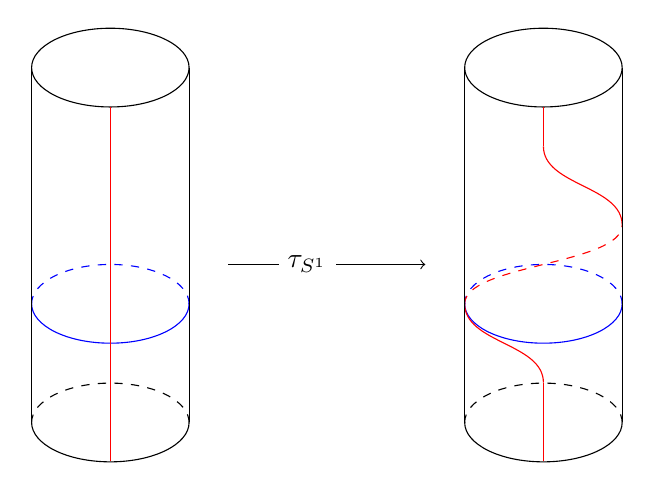
\begin{tikzpicture}

    \begin{scope}[]
    \draw  (-2.5,2.5) ellipse (1 and 0.5);
    
    \begin{scope}[shift={(0,-0.007)}]
    \begin{scope}[]
    
    \clip  (-1.45,-2.55) rectangle (-3.55,-2);
    \draw[]  (-2.5,-2) ellipse (1 and 0.5);
    
    \end{scope}
    \begin{scope}[]
    
    \clip  (-1.45,-1.45) rectangle (-3.55,-2);
    \draw[ dashed]  (-2.5,-2) ellipse (1 and 0.5);
    
    \end{scope}
    \end{scope}\begin{scope}[shift={(0,1.5)}]
    \begin{scope}[]
    
    \clip  (-1.45,-2.55) rectangle (-3.55,-2);
    \draw[blue]  (-2.5,-2) ellipse (1 and 0.5);
    
    \end{scope}
    \begin{scope}[]
    
    \clip  (-1.45,-1.45) rectangle (-3.55,-2);
    \draw[blue, dashed]  (-2.5,-2) ellipse (1 and 0.5);
    
    \end{scope}
    \end{scope}\begin{scope}[shift={(0,0.5)}]
    
    \draw[red] (-2.5,-2) .. controls (-2.5,-1.5) and (-3.5,-1.5) .. (-3.5,-1);
    \draw[red, dashed] (-3.5,-1) .. controls (-3.5,-0.5) and (-1.5,-0.5) .. (-1.5,0);
    \draw[red] (-1.5,0) .. controls (-1.5,0.5) and (-2.5,0.5) .. (-2.5,1);
    \draw[red] (-2.5,-3) -- (-2.5,-2) (-2.5,1) -- (-2.5,1.5);
    \end{scope}
    \draw (-3.5,2.5) -- (-3.5,-2);
    \draw (-1.5,2.5) -- (-1.5,-2);
    \end{scope}
    
    \begin{scope}[shift={(-5.5,0)}]
    \draw  (-2.5,2.5) ellipse (1 and 0.5);
    
    \begin{scope}[shift={(0,-0.007)}]
    \begin{scope}[]
    
    \clip  (-1.45,-2.55) rectangle (-3.55,-2);
    \draw[]  (-2.5,-2) ellipse (1 and 0.5);
    
    \end{scope}
    \begin{scope}[]
    
    \clip  (-1.45,-1.45) rectangle (-3.55,-2);
    \draw[ dashed]  (-2.5,-2) ellipse (1 and 0.5);
    
    \end{scope}
    \end{scope}\begin{scope}[shift={(0,1.5)}]
    \begin{scope}[]
    
    \clip  (-1.45,-2.55) rectangle (-3.55,-2);
    \draw[blue]  (-2.5,-2) ellipse (1 and 0.5);
    
    \end{scope}
    \begin{scope}[]
    
    \clip  (-1.45,-1.45) rectangle (-3.55,-2);
    \draw[blue, dashed]  (-2.5,-2) ellipse (1 and 0.5);
    
    \end{scope}
    \end{scope}
    \draw (-3.5,2.5) -- (-3.5,-2);
    \draw (-1.5,2.5) -- (-1.5,-2);
    \draw[red] (-2.5,2) -- (-2.5,-2.5);
    \end{scope}
    \draw[->] (-6.5,0) -- (-4,0);
    \node[fill=white] at (-5.5,0) {$\tau_{S^1}$};
    \end{tikzpicture}
%label:"thm:seidelDehnTwist"
%author:JeffHicks
%name:"Dehn twist exact sequence"
%type:"theorem"

    Let $X$ be a symplectic manifold, and $S\subset X$ a Lagrangian sphere, and $L\subset X$ another Lagrangian submanifold. There is an exact triangle in the Fukaya category
    \[ \cdots \to \CF(S, L)\otimes S \to L \xrightarrow{\ev} \tau_S(L)\xrightarrow{[1]}\cdots.\]


%tag:000Y
%label:"rem:seidelDehnTwist"
%author:JeffHicks
%name:"Dehn twist exact sequence"
%type:"remark"

    Here, $\CF(S, L)\otimes S$ is a twisted complex. Recall that (as a vector space) $\CF(S, L)=\bigoplus_{x\in S\cap L} \Lambda\langle x \rangle$. 
    The twisted complex $\CF(S, L)\otimes S$ is given by $\bigoplus_{x\in S\cap L} S\langle x \rangle$, which is to say that formal direct sum of copies of $S$ whose grading is determined by the intersection points $x$.
    The differential on a twisted complex is a collection of maps $\delta_{xy}^E\\in \CF(S\langle x \rangle, S\langle y \rangle)$. The morphism we take is 
    \[\delta_{xy}^E= \langle m^1(x), y\rangle \id.\]
    
    We describe the map $\ev: \CF(S, L)\otimes S\to L$. Recall that a morphism of twisted complexes is a collection of maps. We must pick for each $S\langle x \rangle$ a morphism in $\hom(S\langle x \rangle , L)$. Fortunately, there is a canonical choice (which is $x$ itself). 


%tag:000Y
%label:"art:lagrangiancobordisms"
%author:JeffHicks
%name:"lagrangian cobordisms"
%type:"article"

If $M$ is a manifold, a \emph{surgery of $M$} is the replacement of a $D^{n-k}\times S^k$ with $S^{n-k-1}\times D^{k+1}$. 
Surgery of manifolds is closely tied to cobordisms between manifolds. 
Let $M, N$ be $n$-manifolds. 
A \emph{cobordism} $K: M\rightsquigarrow N$ is a manifold with boundary $\partial K=M\sqcup N$. 
There is an analogous notion of cobordism exists for Lagrangian submanifolds.
%label:"def:lagrangianCobordism"
%author:JeffHicks
%name:"differential graded module"
%type:"definition"
%source:"arnol1980lagrange"

Let $\{L_0, \ldots, L_k\}$ be Lagrangian submanifolds of $X$. 
A \emph{Lagrangian cobordism} with positive ends $L_0, \ldots L_k$ is a Lagrangian submanifold $K\subset X\times T^*\RR$ for which there exists a compact subset $D\subset \CC$ so that : 
        \[K\setminus( \pi_\CC^{-1}(D))=\bigcup_{i=0}^k L_i\times \ell_i.\]
    Here, the $\ell_i$ are rays of the form $\ell_i(t)=i\cdot \jmath +t$, where $t\in \RR_{\geq 0}$.
We denote such a cobordism $K:(L_0,L_1, \ldots L_k)\rightsquigarrow \emptyset$. 
\label{def:lagrangianCobordism}


%label:"fig:lagrangianCobordism"
%author:JeffHicks
%name:"Lagragian cobordism"
%type:"figure"
%parent:def:lagrangianCobordism
%caption:"The projection of a Lagrangian cobordism $K\subset X\times \CC$ to the $\CC$ factor. This cobordism has ends  $K:(L_0, L_1, \ldots L_k)\rightsquigarrow \emptyset.$"




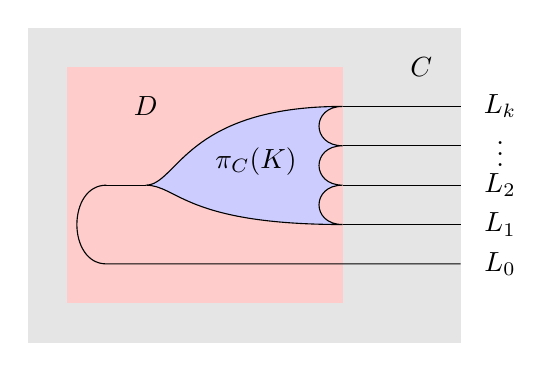
\begin{tikzpicture}[xscale=-1]
    \fill[fill=gray!20]  (-2,-2.5) rectangle (3.5,1.5);
    \fill[red!20]  (-0.5,-2) rectangle (3,1);
        \draw[fill=blue!20] (-0.5,-1) .. controls (-0.1,-1) and (-0.1,-0.5) .. (-0.5,-0.5) .. controls (-0.1,-0.5) and (-0.1,0) .. (-0.5,0) .. controls (-0.1,0) and (-0.1,0.5) .. (-0.5,0.5) .. controls (1.5,0.5) and (1.6,-0.5) .. (2,-0.5) .. controls (1.6,-0.5) and (1.5,-1) .. (-0.5,-1);
        \draw (-2,-1) -- (-0.5,-1);
        \draw (-2,-0.5) -- (-0.5,-0.5);
        \draw (-2,0) -- (-0.5,0);
        \draw (-2,0.5) -- (-0.5,0.5);
        \draw (2,-0.5) -- (2.5,-0.5);
        \node at (-2.5,0.5) {$L_k$};
        \node at (-2.5,0) {$\vdots$};
        \node at (-2.5,-0.5) {$L_2$};
        \node at (-2.5,-1) {$L_1$};
        \node at (-2.5,-1.5) {$L_0$};
        \node at (0.6,-0.2) {$\pi_{\mathbb C}(K)$};
    \draw (2.5,-0.5) .. controls (3,-0.5) and (3,-1.5) .. (2.5,-1.5) .. controls (2,-1.5) and (-1.5,-1.5) .. (-2,-1.5);
    
    \node at (2,0.5) {$D$};
    \node at (-1.5,1) {$\mathbb C$};
    \end{tikzpicture}
%tag:000K
%label:exm:suspensionCobordism
%author:JeffHicks
%name:"suspension of exact homotopy"
%type:example
%source:audin1994symplectic

    Let $\li_s: L\times \RR_t\to X$ be an exact Lagrangian homotopy generated by the function $H_t: L\times \RR_t\to \RR$. 
    The \emph{suspension} of $H_t$ is the Lagrangian cobordism $K_{H_t}$ with topology $L\times \RR$ parameterized by 
    \begin{align*}
          L\times \RR\to & X\times \CC\\
           (u, s)\mapsto& (\li_t(u), s+\jmath H_t(u))\in X\times \CC.
    \end{align*}

%label:"exm:polterovichSurgeryTrace"
%author:JeffHicks
%name:"Polterovich surgery trace"
%type:"example"



    Let $L_1, L_2\subset X$ be Lagrangian submanifolds which intersect transversely at a point $q$, so we can define the Polterovich surgery $L_1\#_q L_2$. 
    Then there exists a Lagrangian cobordism $(L_1\#_U L_2)\rightsquigarrow (L_1, L_2)$. 
    \label{prop:traceconstruction}

%tag:0007
%label:"art:exactSequencesInSymplecticGeometryExercises"
%author:JeffHicks
%name:"Exercises"
%type:"article"


%label:"exr:lagragnianSurgeryOnT2"
%author:JeffHicks
%name:"Lagrangian surgery on $T^2$"
%type:"exercise"

 
 
Consider the torus $T^2=S^1\times S^1$, where we parameterize the circle  $S^1$ as $\RR/\ZZ$. For coprime integers $a, b\in \ZZ$, and $\theta\in S^1$, we write 
\[L_{(a, b),\theta}=\{(a\cdot t+\theta,b\cdot t), t\in S^1\}.\]
for the Lagrangian $S^1$ of slope $(a, b)$ passing through the point $(\theta, 0)$. 
\begin{enumerate}
    \item Compute $\HF(L_{(a, b), \theta_1}, L_{(c, d), \theta_2})$.
    \item Write $L_0:=L_{(1,0), 0}, L_1:= L_{(0,1), 0}$. Let $L_2 = L_0\# L_1$. Find values $(a, b), \theta$ so that $L_2$ is Hamiltonian isotopic to $L_{(a, b), \theta}$.
    \item Let $\{x_{01}\}=L_0\cap L_1$, $\{x_{12}\}=L_1\cap L_2$, and $\{x_{20}\}=L_2\cap L_0$. Prove that 
    \begin{align*}
        m^2(x_{12}, x_{01})=0 && m^2(x_{20}, x_{12})=0 && m^2x_{01}, (x_{20})=0
    \end{align*}
    so that we have what appears to be an exact sequence 
    \[L_0\xrightarrow{x_{01}} L_1 \xrightarrow{x_{12}} L_2 \xrightarrow{x_{20}} L_0[1].\]
    \item What happens in the previous computation if we replace $L_2$ with $L_2'$ which is Lagrangian (but not Hamiltonian) isotopic to $L_2$?
\end{enumerate}



 
%tag:0014
%label:"exr:dehnTwistAsSurgery"
%author:JeffHicks
%name:"Dehn twist as surgery"
%type:"exercise"

 
 
Consider the space $T^*S^n$ which we describe as a symplectic submanifold of $T^*S^n$ by the equation
\[\{(x_0, \ldots, x_n), (p_0, \ldots, p_n) \st \sum_{i} (x_i+\sqrt{-1} p_i)^2=1 \}\]
\begin{enumerate}
    \item Consider the Hamiltonian given by $H=|\vec p|^2$. Write down the Hamiltonian vector field on $T^*S^n$, and compute its time-one flow.
    \item Consider now the symplectic manifold with boundary 
    \[B^*_1S^n=\{(x_0, \ldots, x_n), (p_0, \ldots, p_n) \st\vec x\cdot \vec p =0,|\vec x|=1, |\vec p|<1\}.\]
    Show that $\phi_{2\pi}: B^*_1S^n\to B^*_1 S^n$, the time-1 Hamiltonian flow of $|\vec p|^2$, acts by  $-1$ on the boundary of $B^*_1S^n$. 
    \item The symplectic Dehn twist is the map: 
    \begin{align*}
        \tau^n: B^*_1 S^n\to& B^*_1 S^n\\
            (\vec x, \vec p) \mapsto& -\phi_{\pi}(\vec x, \vec p).
    \end{align*}
    which fixes the boundary of $B^*_1 S^n$.
    Consider the Lagrangian submanifold  
    \[F_q:=\{(1, \ldots, 0), (0, p_1, \ldots, p_n)\}\subset B^*_1S^n.\]
    Show that there is a Hamiltonian isotopy which identifies
    \[\tau_n(F_q)\sim S^n\# F_q.\]
    \item Consider in $T^2$ the Lagrangian submanifold $L:=L_{(1, 0),0}$ as before. Identify a small neighborhood $U$ of $L$ with $B^*_1(S^1)$, and define\footnote{This does not quite give a smooth map, but it can be made smooth by slightly modifying the definition of $\tau^n$.} $\tau_L: T^2\to T^2$ by 
    \[\tau_L(x)=\left\{\begin{array}{cc} \tau^1(x) &\text{if $x\in U$}\\
        x &\text{otherwise}\end{array}\right.\]
    For $a, b\in \ZZ$, and $\theta\in S^1$, find the Lagrangian submanifold $L_{(a', b'), \theta'}$ which is Hamiltonian isotopic to  $\tau_L(L_{(a, b), \theta})$.
\end{enumerate}

 
%label:"exr:biranCornea3ended"
%author:JeffHicks
%name:"surgery triangle from Lagrangian cobordism"
%type:"exercise"

 
 
Let $X$ be a compact symplectic manifold. Recall that a \emph{3-ended Lagrangian cobordism} $K: (L_0, L_1)\rightsquigarrow L_2$ is a closed Lagrangian submanifold $K\subset X\times \CC$ with the property that there exists a compact subset $U\subset \CC$ so that \[K|_{\pi_\CC^{-1}(\CC\setminus U)}=((L_0\times \RR_{>0})\cup( L_1\times (\sqrt{-1}+\RR_{>0}) )\cup( L_2\times (\RR_{<0})))|_{\pi_\CC^{-1}(\CC\setminus U)}.\]
Suppose that $X$ is an exact symplectic manifold, which in turn makes $X\times \CC$ an exact symplectic manifold. Let $K$ be an exact 3-ended Lagrangian cobordism. 
    %label:"fig:3EndedLagrangianCobordism"
%author:JeffHicks
%name:"3 ended Lagrangian cobordism"
%type:"figure"
%parent:"exr_biranCornea3ended"
%caption:"The projection to the $\CC$ coordinate of a 3-ended Lagrangian cobordism"


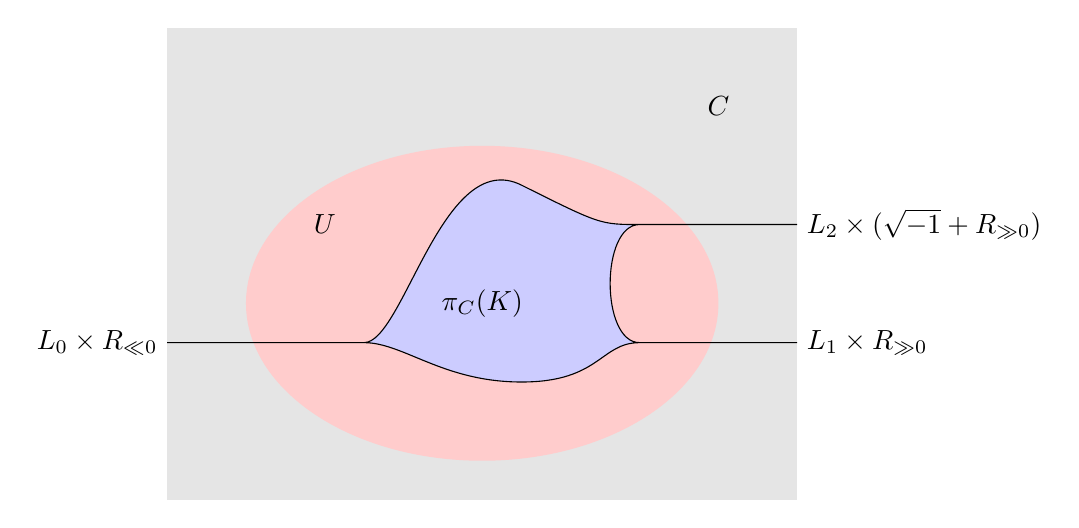
\begin{tikzpicture}

\fill[gray!20]  (-3.5,2.5) rectangle (4.5,-3.5);
\fill[fill=red!20]  (0.5,-1) ellipse (3 and 2);

\draw[fill=blue!20] (-3.5,-1.5) .. controls (-3,-1.5) and (-1.5,-1.5) .. (-1,-1.5) .. controls (-0.5,-1.5) and (0,-2) .. (1,-2) .. controls (2,-2) and (2,-1.5) .. (2.5,-1.5) .. controls (3,-1.5) and (4,-1.5) .. (4.5,-1.5) .. controls (4,-1.5) and (3,-1.5) .. (2.5,-1.5) .. controls (2,-1.5) and (2,0) .. (2.5,0) .. controls (3,0) and (4,0) .. (4.5,0) .. controls (4,0) and (3,0) .. (2.5,0) .. controls (2,0) and (2,0) ..(1,0.5) .. controls (0,1) and (-0.5,-1.5) .. (-1,-1.5);
\node[left] at (-3.5,-1.5) {$L_0\times \mathbb R_{\ll 0}$};
\node[right] at (4.5,-1.5) {$L_1\times \mathbb R_{\gg 0}$};
\node[right] at (4.5,0) {$L_2\times(\sqrt{-1}+ \mathbb R_{\gg 0})$};
\node at (0.5,-1) {$\pi_{\mathbb C}(K)$};
\node at (3.5,1.5) {$\mathbb C$};
\node at (-1.5,0) {$U$};
\end{tikzpicture}

\begin{enumerate}
    \item Show that $L_0, L_1$ and $L_2$ are exact Lagrangian submanifolds in $X$.
    \item Consider the curve $\gamma^-\subset \CC$. Show that for any exact Lagrangian submanifold $L\subset X$, $\CF(L\times \gamma^-, K)=\CF(L, L_0)$ as a vector space. 
    \item Give $X\times \CC$ an almost complex structure of the form $J_X\times J_\CC$. Suppose that we have a finite energy pseudoholomorphic strip $u: \RR\times [0, 1]\to X\times \CC$ with $u(t, 0)\in L\times \gamma^-$ and $u(t, 1)\in K$, and ends limiting to intersections of $L\times \gamma^-\cap K$. Show that $\pi_\CC(u)\in \text{Im}(\gamma^-)\cap \RR_{<0}$ (the location of the red cross in the figure). From this, conclude that if $J_X$ is chosen so that all pseudoholomorphic strips with boundary on $L, L_2$ are regular, that $\CF(L\times \gamma^-, K) = \CF(L_2, K)$ \emph{as chain complexes}.
        %tag:000X
%label:"fig:3EndedLagrangianCobordismGammaMinus"
%author:JeffHicks
%name:"3 ended Lagrangian cobordism with curve $\gamma^-$"
%type:"figure"
%parent:exr_biranCornea3ended
%caption:"Profile of the curve $\gamma^-$"


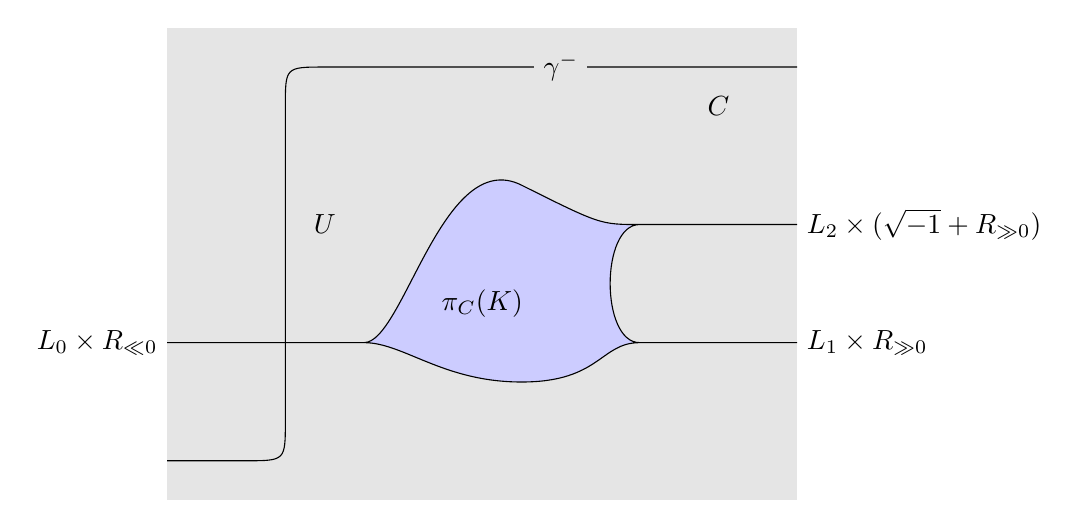
\begin{tikzpicture}

\fill[gray!20]  (-3.5,2.5) rectangle (4.5,-3.5);

\draw[fill=blue!20] (-3.5,-1.5) .. controls (-3,-1.5) and (-1.5,-1.5) .. (-1,-1.5) .. controls (-0.5,-1.5) and (0,-2) .. (1,-2) .. controls (2,-2) and (2,-1.5) .. (2.5,-1.5) .. controls (3,-1.5) and (4,-1.5) .. (4.5,-1.5) .. controls (4,-1.5) and (3,-1.5) .. (2.5,-1.5) .. controls (2,-1.5) and (2,0) .. (2.5,0) .. controls (3,0) and (4,0) .. (4.5,0) .. controls (4,0) and (3,0) .. (2.5,0) .. controls (2,0) and (2,0) ..(1,0.5) .. controls (0,1) and (-0.5,-1.5) .. (-1,-1.5);
\node[left] at (-3.5,-1.5) {$L_0\times \mathbb R_{\ll 0}$};
\node[right] at (4.5,-1.5) {$L_1\times \mathbb R_{\gg 0}$};
\node[right] at (4.5,0) {$L_2\times(\sqrt{-1}+ \mathbb R_{\gg 0})$};
\node at (0.5,-1) {$\pi_{\mathbb C}(K)$};
\node at (3.5,1.5) {$\mathbb C$};
\node at (-1.5,0) {$U$};
\draw (-3.5,-3) .. controls (-3,-3) and (-3,-3) .. (-2.5,-3) .. controls (-2,-3) and (-2,-3) .. (-2,-2.5) .. controls (-2,-2) and (-2,1) .. (-2,1.5) .. controls (-2,2) and (-2,2) .. (-1.5,2) .. controls (-1,2) and (4,2) .. (4.5,2);
\node[fill=gray!20] at (1.5,2) {$\gamma^-$};
\end{tikzpicture}
    \item Consider now the curve $\gamma^+\subset \CC$. Using a similar argument, one can prove that there are no pseudoholomorphic strips $u:\RR\times [0, 1]\to X\times \CC$ with $\lim_{t\to\infty} u(s, t)=z_2$ and $\lim_{t\to-\infty} u(s, t)=z_0$. What can you conclude about the relationship between $\CF(L\times \gamma^+, K)$, $\CF(L, L_0)$ and $\CF(L, L_1)$?
        \input{fig_3EndedLagrangianCobordismGammaPlus}
    \item Observe that $L\times \gamma^-$ and $L\times \gamma^+$ are Hamiltonian isotopic. Exhibit a long exact sequence whose terms are $\HF(L, L_0), \HF(L, L_1)$ and $\HF(L, L_2)$.
\end{enumerate}

 

    \end{exposition}